%%%%%%%%%%%%%%%%%%%%%%%%%%%%%%%%%%%%%%%%%%%%%%%%%%%%%%%%%%%%%%%%%%%%%%%%%%%%%%%%%%
%%																				%%
%% File name: 		main.tex													%%
%% Project name:	Applications in Deep Learning								%%
%% Type of work:	Advanced Seminar											%%
%% Author:			Hannes Bohnengel											%%
%% Mentor:			Debayan Roy													%%
%% Date:			07 July 2017												%%
%% University:		Technical University of Munich								%%
%% Comments:		Created in texstudio with tab width = 4						%%
%%																				%%
%%%%%%%%%%%%%%%%%%%%%%%%%%%%%%%%%%%%%%%%%%%%%%%%%%%%%%%%%%%%%%%%%%%%%%%%%%%%%%%%%%

%---- Define document class ------------------------------------------------------

% copied acmart.cls to /usr/share/texlive/texmf-dist/tex
\documentclass[format=sigconf, review=false, screen=false, timestamp=false, authordraft=false, 9pt]{acmart}

%---- Define used packages -------------------------------------------------------

\usepackage{mypaper}

%---- Begin of document ----------------------------------------------------------

\begin{document}
	
	% To adjust the spacing (default: 1)
	\renewcommand{\baselinestretch}{1}
	
	% Title portion. Note the short title for running heads 
	\title{The Impact of Deep Learning on \\Speech Synthesis with Mobile Devices}  
%	\subtitle{A Systematic Review}
	\author{Hannes Bohnengel}
	%\orcid{1234-5678-9012-3456}
	\affiliation{%
		\institution{Technical University of Munich}
		%\streetaddress{104 Jamestown Rd}
		%\city{Williamsburg}
		%\state{VA}
		%\postcode{23185}
		%\country{USA}
		}
	\email{hannes.bohnengel@tum.de}	

%---- Adjust some layout stuff ---------------------------------------------------
	
	% Paper margins
	\newgeometry{left=1.78cm,right=1.78cm,top=1.4cm,bottom=1.7cm, footskip=1cm}
	
	% This is the default geometry:
	%\geometry{twoside=true, head=13pt, paperwidth=8.5in, paperheight=11in, includeheadfoot, columnsep=2pc, top=57pt, bottom=73pt, inner=54pt, outer=54pt, marginparwidth=2pc}
	
	% Column spacing
	\setlength{\columnsep}{0.8cm}
	
%---- Input abbreviations ---------------------------------------------------------			

% !TeX root = ../main.tex

%%%%%%%%%%%%%%%%%%%%%%%%%%%%%%%%%%%%%%%%%%%%%%%%%%%%%%%%%%%%%%%%%%%%%%%%%%%%%%%%%%
%%																				%%
%% File name: 		abbreviations.tex											%%
%% Project name:	Applications in Deep Learning								%%
%% Type of work:	Advanced Seminar											%%
%% Author:			Hannes Bohnengel											%%
%% Mentor:			Debayan Roy													%%
%% Date:			23 May 2017													%%
%% University:		Technical University of Munich								%%
%% Comments:		Created in texstudio with tab width = 4						%%
%%																				%%
%%%%%%%%%%%%%%%%%%%%%%%%%%%%%%%%%%%%%%%%%%%%%%%%%%%%%%%%%%%%%%%%%%%%%%%%%%%%%%%%%%

% List of acronyms

\newacro{ASR} {automatic speech recognition}
\newacro{DNN} {deep neural network}
\newacro{HMM} {hidden Markov model}
\newacro{IoT} {internet of things}
\newacro{SPSS}{statistical parametric speech synthesis}
\newacro{SPSG}{statistical parametric speech generation}
\newacro{VPA}{virtual personal assistant}


% Alternative command:
%\acrodef{SPSS}{statistical parametric speech synthesis}	
	
%---- Input abstract text --------------------------------------------------------			
	
	% !TeX root = ../main.tex

%%%%%%%%%%%%%%%%%%%%%%%%%%%%%%%%%%%%%%%%%%%%%%%%%%%%%%%%%%%%%%%%%%%%%%%%%%%%%%%%%%
%%																				%%
%% File name: 		abstract.tex												%%
%% Project name:	Applications in Deep Learning								%%
%% Type of work:	Advanced Seminar											%%
%% Author:			Hannes Bohnengel											%%
%% Mentor:			Debayan Roy													%%
%% Date:			11 June 2017												%%
%% University:		Technical University of Munich								%%
%% Comments:		Created in texstudio with tab width = 4						%%
%%																				%%
%%%%%%%%%%%%%%%%%%%%%%%%%%%%%%%%%%%%%%%%%%%%%%%%%%%%%%%%%%%%%%%%%%%%%%%%%%%%%%%%%%

\begin{abstract}
	In this paper I aim to give a systematic review about the impact of deep learning-based implementation of speech synthesis systems on resource restricted devices. First a brief introduction into \ac{SPSS} and its alternatives is given, then two approaches on how to improve \ac{SPSS} with deep learning models are presented. 
	%Therefore the performance and quality is compared to conventional systems.
\end{abstract}

%---- Input keywords -------------------------------------------------------------			

	%\keywords{\textbf{\color{ACMRed}NECESSARY???} Deep Learning, Deep Neural Network, Embedded System, Mobile Device, Speech Synthesis, Text-to-Speech}
		
	\maketitle
	
	% If the default list of authors is too long for headers}
	%\renewcommand{\shortauthors}{H.Bohnengel}
	
%---- Input main text -------------------------------------------------------------		
	
	
	\vspace{-0.5em}
	
	% !TeX root = ../main.tex

%%%%%%%%%%%%%%%%%%%%%%%%%%%%%%%%%%%%%%%%%%%%%%%%%%%%%%%%%%%%%%%%%%%%%%%%%%%%%%%%%%
%%																				%%
%% File name: 		introduction.tex											%%
%% Project name:	Applications in Deep Learning								%%
%% Type of work:	Advanced Seminar											%%
%% Author:			Hannes Bohnengel											%%
%% Mentor:			Debayan Roy													%%
%% Date:			23 May 2017													%%
%% University:		Technical University of Munich								%%
%% Comments:		Created in texstudio with tab width = 4						%%
%%																				%%
%%%%%%%%%%%%%%%%%%%%%%%%%%%%%%%%%%%%%%%%%%%%%%%%%%%%%%%%%%%%%%%%%%%%%%%%%%%%%%%%%%



\section{Introduction}

Virtual personal assistants (\acsu{VPA}) like Siri, Cortana or Google Now start having a huge impact on the way of interacting with electronic devices like smartphones or notebooks. Up to now the \acp{VPA} help only with rather simple tasks like search queries, starting phone calls or setting a clock, but according to a recent survey from the IT research firm Gartner~\cite{gartner:assistants}, this will change in the near future. With the Facebook Messenger it is already possible to make purchases or to order a Uber car and here new use cases are expected soon. The survey also states, that through the vastly increase of devices in the scope of the \ac{IoT} the way of interacting with machines will go towards minimal or zero touch. Instead of interacting through common touch-displays or buttons, the user simply speaks to the device, like to another person. To enable this, both \ac{ASR} and speech synthesis are essential technologies.

In this paper I will only focus on the speech synthesis part. A widley spread technique to synthesize human speech from a given text or from linguistic descriptions is \ac{SPSS}; also referred to as \ac{SPSG} \cite{ling:deep}. This technique is based on the usage of \acp{HMM}. Zen \textsl{et al.} \cite{zen:statistical} show that it has several advantages over its predecessor, the concatenative speech synthesis, for example the flexibility in changing voice characteristics and a smaller memory footprint. However the quality of the generated speech still has potential for improvement. Due to over-smoothing the voice sounds muffled in comparison to natural speech.

This is where recent achievements in deep learning come in. Deep learning is usually referred to as a class of machine learning techniques that achieve tasks like feature extraction or pattern analysis by using many connected layers of non-linear information processing \cite{ling:deep, li:survey}. Since 2006 ...

In \cite{li:survey} the author states four different approaches to improve \ac{SPSS} through deep learning models: 

\newpage

\begin{enumerate}
	\item Why speech synthesis is important? What are its applications?
	\item What are the conventional techniques of speech synthesis? What are the drawbacks of such techniques?
	\item What is deep learning? What improvements do deep learning algorithms bring?
	\item How some algorithms are modified to suit speech synthesis?
	\item Why is it important to implement speech synthesis on embedded platform?
	\item An example of how speech synthesis can be implemented on embedded platform without deep learning.
	\item How the 3 can be combined?
	\item Future works.
\end{enumerate}


These are the core papers: 
\begin{itemize} %%{label}{spacing}
	\item Robust Deep-learning Models for Text-to-speech Synthesis Support on Embedded Devices \cite{boros:robust}
	\item Statistical parametric speech synthesis using deep neural networks \cite{zen:deepstatistical}
	\item Deep neural networks employing Multi-Task Learning and stacked bottleneck features for speech synthesis \cite{wu:deep}
	\item Efficient deep neural networks for speech synthesis using bottleneck features \cite{joo:efficient}
	\item On the training aspects of Deep Neural Network (DNN) for parametric TTS synthesis \cite{qian:training}
	\item TTS synthesis with bidirectional LSTM based recurrent neural networks \cite{fan:tts}
	\item The effect of neural networks in statistical parametric speech synthesis \cite{hashimoto:effect}
	\item Efficient memory compression in deep neural networks using coarse-grain sparsification for speech applications \cite{kadetotad:efficient}
	\item Speeding up deep neural networks for speech recognition on ARM Cortex-A series processors \cite{xing:speeding}
\end{itemize}

These are interesting references:

\begin{itemize} %%{label}{spacing}
	\item Deep Learning for Acoustic Modeling in Parametric Speech Generation: A systematic review of existing techniques and future trends \cite{ling:deep}
	\item A tutorial survey of architectures, algorithms, and applications for deep learning \cite{li:survey}
\end{itemize}

%\newpage
\clearpage
	
	% !TeX root = ../main.tex

%%%%%%%%%%%%%%%%%%%%%%%%%%%%%%%%%%%%%%%%%%%%%%%%%%%%%%%%%%%%%%%%%%%%%%%%%%%%%%%%%%
%%																				%%
%% File name: 		body.tex													%%
%% Project name:	Applications in Deep Learning								%%
%% Type of work:	Advanced Seminar											%%
%% Author:			Hannes Bohnengel											%%
%% Mentor:			Debayan Roy													%%
%% Date:			07 June 2017												%%
%% University:		Technical University of Munich								%%
%% Comments:		Created in texstudio with tab width = 4						%%
%%																				%%
%%%%%%%%%%%%%%%%%%%%%%%%%%%%%%%%%%%%%%%%%%%%%%%%%%%%%%%%%%%%%%%%%%%%%%%%%%%%%%%%%%

\section{Conventional Speech Synthesis}
\label{sec:speech}

\subsection{Motivation \& Approaches}
\label{subsec:convenspeech}

Speech synthesis has emerged over the last 10 years due to a vast contribution by the global community of researchers and the increasing computational power for data processing. Its quality and naturalness has increased steadily and different approaches have been developed so far \cite{suendermann:challenges}. The typical applications like navigation systems in cars or telephone-based dialogue systems are nowadays widely established. But also as reading aid for visually impaired people \cite{readspeaker:tts} or as in the case of the famous scientist Stephen Hawking, who has been using a synthesized voice to communicate since 1997 \cite{hawking:speech}, speech synthesis has proven to be very useful. Another very interesting application of speech synthesis is shown in [XX]. The author proposed to introduce synthetic speech as means of communication between pilots, since there have been many accidents due to missunderstandings at radio-based communication. %Finally the interaction between man and machines or robots \cite{hill:manmachine}

According to \cite{hinterleitner:quality} speech synthesis can be divided into three types: Canned speech, \ac{CTS} and \ac{TTS}. Canned speech more or less is the replay of prerecorded spoken sentences or words with none or very little adjustments. A typical example are the announcements on train stations. Because of the high effort of recording everything (almost) exactly as it is replayed, this approach is limited to only a few simple applications. With \ac{CTS} the waveform is generated out of a linguistic description without any information of the respective text. In this way no natural language processing is required, but nevertheless \ac{CTS} nowadays has not made any important impact. The last and most promising type is \ac{TTS}.

A \ac{TTS} system consists of a \ac{NLP} part, where the text is analysed and the word and sentence structure and accents are extracted. In the next step these accents are used to generate the prosody of the given text like duration, intensity and pitch. Then the created phonetic represantations with prosody information are stringed together to a continuous stream of signal parameters. The last task, the speech generation, uses this stream to generate the respective waveform. This function block can be implemented in different ways. In \cite{hinterleitner:quality} three general approaches are named as follows: Parametric Speech Synthesis (formant-based synthesis), Concatenative Speech Synthesis (unit-selection synthesis) and Statistical Parametric Speech Synthesis (\ac{HMM}-based synthesis). The methods in brackets are the respective implementations, which are most commonly used. 

The formant-based synthesis is the oldest approach. To generate a voice waveform, an excitation signal is fed into multiple formant filters which describe the characteristics of the human vocal tract. The output of the filters then forms the voice waveform. This technique is the only one which does not need any recorded speech, but instead generates the synthesized voice only by modeling the human vocal tract. The quality of the generated voice is the lowest in comparison to the other techniques, but therefore formant-based synthesizer have the smallest footprint and the voice characteristics can easilily been modified by just changing the filter parameters~\cite{hinterleitner:quality}.

With the development of concatenative speech synthesizer the quality of the generated speech improved tremendously. Very similar to \ac{CTS} prerecorded speech is used as reference. Very basically said, the recorded speech is devided into units and these units are then stringed together to form the new speech signal according to a given text. Hereby the chosen size of the units determines both the footprint size and the voice quality. With larger units a higher voice quality can be achieved, but this also results in a much larger database. The challenge in unit-selection is to ensure, that the transissions between the units are as natural as possible~\cite{hinterleitner:quality}. In Section~\ref{subsec:hmmspeech} some concepts on how to achieve this as well as the third implementation, the \ac{HMM}-based synthesis, a specific instance of \ac{SPSS} are described in detail.

\subsection{\ac{HMM}-based Speech Synthesis}
\label{subsec:hmmspeech}

In this section the \ac{HMM}-based, the most recent approach for speech synthesis will be described further and both advantages and drawbacks compared to unit-selection synthesis will be highlighted. Therefore the work of Black \textit{et al.} \cite{black:statistical} will be taken as reference.

The quality of unit-selection synthesis directly depends from the quality of the prerecorded speech. But even with a database of excellent quality sporadic errors can still not be avoided totally. If a specific phonetic or prosodic part of a generated sentence is not well represented in the database the output quality of this sentence suffers immensely. To try to avoid this a huge effort in specifically designing the database for the required application can be performed, but still there is no guarantee that such bad joins happen. In addition the fact, that in unit-selection no or only very little adaptions of the voice characteristics are possible without an enormous increase of the database size, the ambition towards seamless speech synthesis leads to the \ac{HMM}-based approach. There a statistic representation of some sets of speech segments is used to generate arbitrary synthetic speech.

\textbf{{\color{ACMRed}Details about unit-selection synthesis ???}}

In Figure~\ref{fig:hmm} the structure of a typical \ac{HMM}-based synthesizer is shown. The whole system can be devided into two parts, the training and the synthesis part. The connection of these two parts is a set of context-dependent ({\color{ACMRed}what is that?}) \acp{HMM}. In the training part spectrum and excitation parameters of the recorded speech are used to generate acoustic models represented by the \acp{HMM}. Thereby phonetic, linguistic and prosodic parameters are considered. {\color{ACMRed}Details about spectrum and excitation parameters?} In comparison to a unit-selection system the database only is needed in the training part.

\begin{figure}[h]
	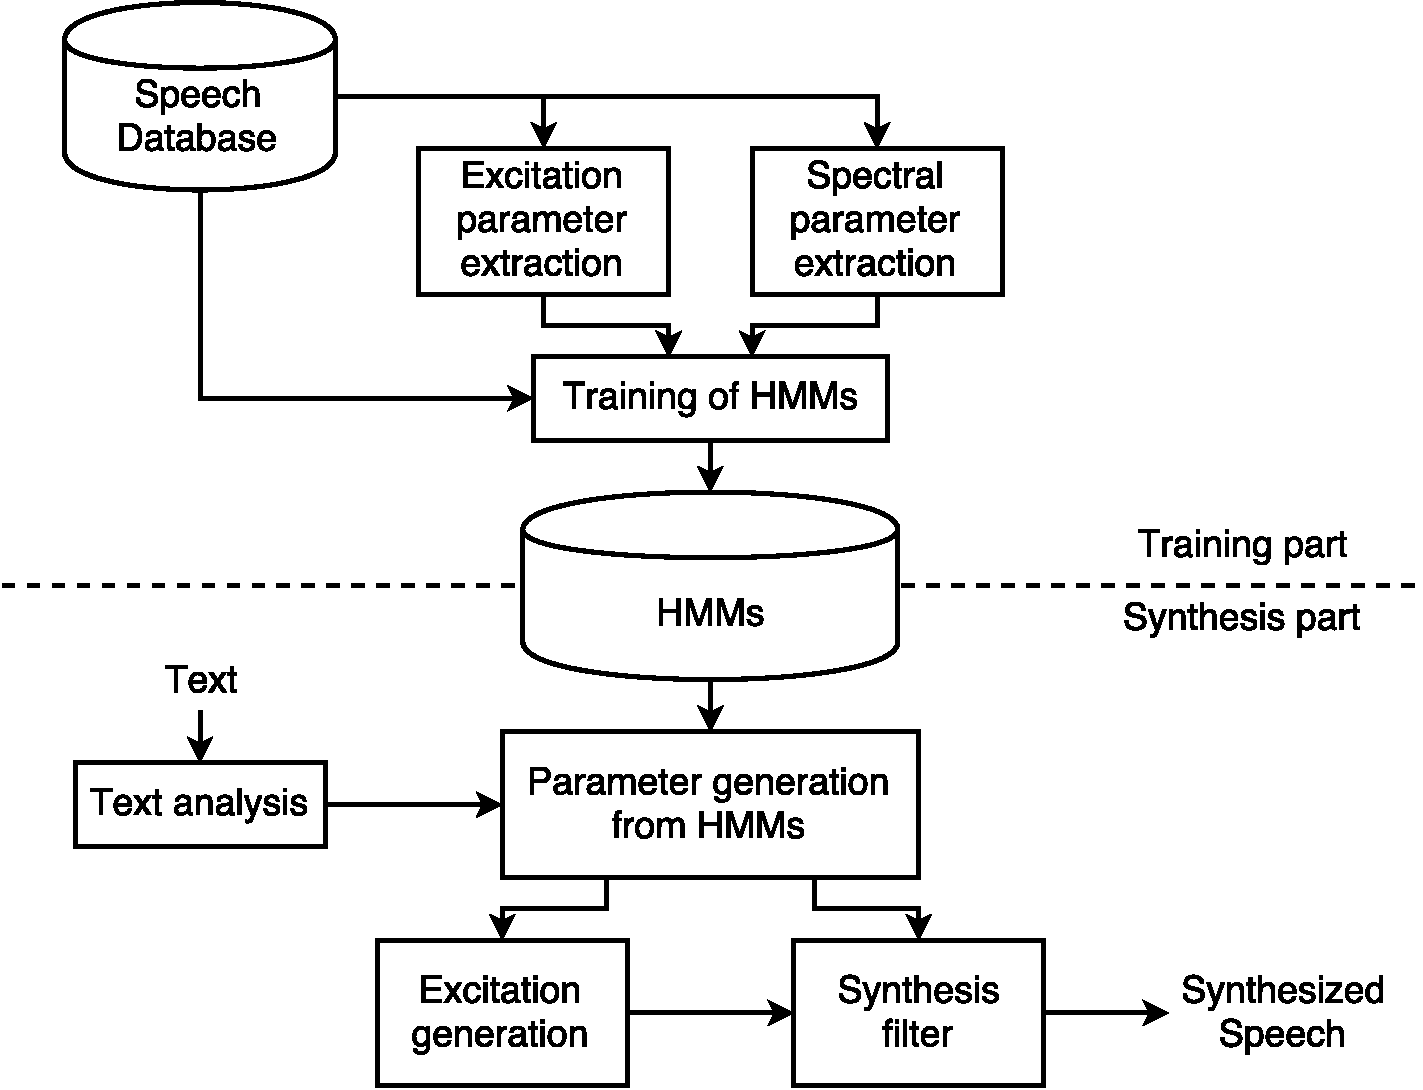
\includegraphics[width=0.8\columnwidth]{hmm-system.pdf}
	\caption{Function blocks of \ac{HMM}-based synthesis \cite{black:statistical}}
	\label{fig:hmm}
\end{figure}

In the synthesis part first the text which is to be synthesized is transformed to a sequence of parameters containing information about the context ({\color{ACMRed}what context?}). According to this sequence the respective \acp{HMM} ({\color{ACMRed}what is that?}) are concatenated in order to form an utterance \ac{HMM}. Then after determining the state durations of the \acp{HMM} a sequence of coefficients is created, which finally is used to construct the speech waveform using a special filter ({\color{ACMRed}details?}).

The main disadvantage of this approach compared to unit-selection synthesis is the quality of the synthesized speech. Three factors are accountable for the lack of quality: the vocoder, the modeling accuracy, and an effect called over-smoothing ({\color{ACMRed}details?}).

However there are some essential advantage, which makes the \ac{HMM}-based approach a competitive alternative to unit-selection synthesis. First, the voice characteristics can be modified without much effort Thus the implementation of different languages and the realization of different speaking styles with emotional emphasize is possible. Second, these just named aspects require a much smaller database than in unit-selection synthesis, since only a statistic represantation of speech segments rather than raw speech data is stored. 

In Table~\ref{tab:speechgeneration} the up to here mentioned techniques are compared regarding the most prominent advantages and drawbacks.

\begin{table}[h]
	\caption{Comparison of speech generation methods~\cite{hinterleitner:quality, black:statistical}}
	\label{tab:speechgeneration}
	\begin{tabularx}{1\columnwidth}{cYY}
		\toprule
		\textbf{Technique} & \textbf{Advantages} & \textbf{Drawbacks}\\
		\midrule
		Formant-based & No prerecorded speech required & Very artificial and metallic voice\\[0.5em]
		Unit-selection & Very high voice quality possible & Large database required\\[0.5em]
		\ac{HMM}-based & Adjustable voice and small footprint & Voice sounds muffled\\
		\bottomrule
	\end{tabularx}
\end{table}

\begin{itemize}[leftmargin=10pt]
	\bfseries\color{ACMRed}
	\item (Relationship between the two approaches)
	\item (Hybrid approaches)
	\item Why there is need to further improve this technology?
	\item What is a HMM?
	\item Bring up MLPG (Maximum Likelyhood Parameter Generation)
	\item Bring up Decision Tree
	\item Robustness as additional advantage (source [10] in \cite{zen:deepstatistical})
\end{itemize}

%---------------------------------------------------------------------------------
%---------------------------------------------------------------------------------
% SPSS with Deep Learning Models
%---------------------------------------------------------------------------------
%---------------------------------------------------------------------------------

\section{\ac{SPSS} with Deep Learning Models}
\label{sec:deepspeech}

{\color{ACMRed}In this section first different approaches of deploying deep learning models are investigated, as shown in \cite{hashimoto:effect} and then one specific approach is explained further, wherefore \cite{zen:deepstatistical} is used as reference.}

\subsection{One specific approach for improvement}
\label{subsec:deepspss}

In the previous section we learned that the quality issue of \ac{HMM}-based speech synthesis is caused by three aspects, the vocoder, the accuracy of acoustic models and the over-smoothing effect. Zen \textit{et al.} \cite{zen:deepstatistical} suggest a specific approach to eliminate one of these causes, the accuracy of acoustic models, by allocating this task to a \ac{DNN}. In convential \ac{HMM}-based systems the mapping between context features (phonetic and linguistic properties) and speech parameters is done by decision tree based context clustering. Thereby the context-dependent \acp{HMM} are assigned to different clusters depending on the combination of contexts using binary decision trees. Each cluster is characterized by a specific set of speech parameters. In this way it is possible to estimate all \acp{HMM} in a robust way, with a typically sized training database.

However decision trees soon reach their limits when handling complex contexts. Only by increasing the size and in this way decreasing the efficiency of the decision tree more complicated contexts (e.g. XOR) can be dealt with. 

In addition to that decision require partitioned input data with each partition having a different set of parameters. In this way whith less data per region overfitting (weak generalization) is likely to happen, which then results in a lack of quality. These downsides can be avoided by using a \ac{DNN} instead of multiple decision trees.

But the use of a \ac{DNN} also introduces two disadvantages: The first one arises in terms of computational power. Both in the training and in the prediction stage decision trees require much less operations (total amount and level of complexity) than \acp{DNN}. The second one has to do with the decision process in its basic form. With decision trees a binary question has to be answered, whilst a \ac{DNN} consists of weighted neurons, which use non-linear activation functions (e.g. \textit{sigmoid}, \textit{tanh}, \textit{ReLU} \cite{chung:activation}) to determine their state. As consequence of that interpretable rules are far easier to produce with decision trees, than with \acp{DNN}.

In Figure~\ref{fig:dnnspeech} the structure of a \ac{DNN}-based speech synthesis system is shown. First a sequence of input features is generated after analysing the input text. These parameters contain numeric values like the number of words in a sentence or the duration of a phoneme as well as binary answers to questions like ,,is the current phoneme \textit{aa}?''. Then this parameter sequence is fed into the \ac{DNN} where a mapping to output features is deployed by using forward propagation. The \ac{DNN} has to be trained sometime before with pairs of input and output features from a database. In the following steps the speech parameters are extracted from the statistics of the output features and the voice waveform in turn generated from the speech parameters. this is done in the same way as in the \ac{HMM}-based system. For this system the function blocks of text analysis, parameter generation, and waveform synthesis can be reused from a \ac{HMM}-based system. Only the mapping from input features (e.g. linguistic contexts) to output features (spectral and excitation parameters) is implemented in a different way.

\begin{figure}[h]
	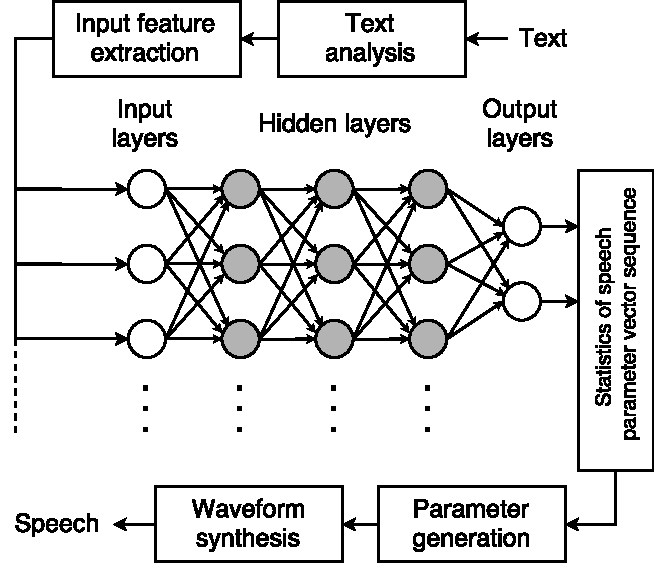
\includegraphics[width=0.9\columnwidth]{dnn-speech-small.pdf}
	\caption{Speech synthesis based on \ac{DNN} \cite{zen:deepstatistical}}
	\label{fig:dnnspeech}
\end{figure}

Experiments and results: Objective and subjective evaluation; DNNs with different number of units/layer (256- 2048)

\vspace{5em}


\begin{table}[h]
	\caption{Subjective scores (in \%) of speech samples in  ~\cite{zen:deepstatistical}}
	\label{tab:subeval}
	\begin{tabularx}{0.7\columnwidth}{cYc}
		\toprule
		\textbf{\ac{HMM}} & \textbf{\ac{DNN}} & \textbf{Neutral}\\
		($\alpha$) & (layers $\times$ units) & \\
		\midrule
		15.8 (16) & 38.5 (4 $\times$ 256) & 45.7\\[0.5em]
		16.1 (4) & 27.2 (4 $\times$ 512) & 56.8\\[0.5em]
		12.7 (1) & 36.6 (4 $\times$ 1\,024) & 50.7\\
		\bottomrule
	\end{tabularx}
\end{table}

Conclusions: Improved performance for predicting spectral and excitation parameters. More natural sounding voice. BUT: Higher computational costs both at training and prediction stage.

\newpage

\subsection{Other ways for improvement}
\label{subsec:deepeffect}

Although, the approach of \ac{SPSS} has brought many advantages over unit-selection synthesis, as shown in the previous section, the generated voice is still not as natural as desired. Therfore deep learning models recently have been used to further improve \ac{SPSS}. Since \acp{DNN} have proven to be very effective in speech recognition, they have found their way into speech synthesis. With the use of \acp{DNN} it is possible to represent higher dimensional and correlated features in an efficient way as well as compactly modeling complex mapping functions. Exactly these properties can be used in \ac{SPSS}, where different features representing the context (linguistic, prosody, etc.) have to be considered for the acoustic modeling \cite{hashimoto:effect}.

In \cite{hashimoto:effect} the effects of deep learning methods on \ac{SPSS} are investigated. Therefore the different parts of a \ac{HMM}-based speech synthesis system are modeled with a \ac{DNN} and then the output is compared to the conventional approach.

-> \textbf{other approach than DNN as acoustic model as in \cite{zen:deepstatistical}}

\newpage

%---------------------------------------------------------------------------------
%---------------------------------------------------------------------------------
% Speech Synthesis on Embedded Devices
%---------------------------------------------------------------------------------
%---------------------------------------------------------------------------------

\section{Speech Synthesis on Embedded Devices}
\label{sec:embeddedspeech}

\subsection{Motivation}
\label{subsec:motembedded}

Why is it important to implement speech synthesis on embedded platform?\\
What needs to be thought about when dealing with embedded or mobile devices?

\subsection{\ac{HMM}-based Approach}
\label{subsec:hmmembedded}

\subsection{Deep Learning-based Approach}
\label{subsec:deepembedded}

\clearpage

	
	% !TeX root = ../main.tex

%%%%%%%%%%%%%%%%%%%%%%%%%%%%%%%%%%%%%%%%%%%%%%%%%%%%%%%%%%%%%%%%%%%%%%%%%%%%%%%%%%
%%																				%%
%% File name: 		conclusion.tex												%%
%% Project name:	Applications in Deep Learning								%%
%% Type of work:	Advanced Seminar											%%
%% Author:			Hannes Bohnengel											%%
%% Mentor:			Debayan Roy													%%
%% Date:			01 June 2017												%%
%% University:		Technical University of Munich								%%
%% Comments:		Created in texstudio with tab width = 4						%%
%%																				%%
%%%%%%%%%%%%%%%%%%%%%%%%%%%%%%%%%%%%%%%%%%%%%%%%%%%%%%%%%%%%%%%%%%%%%%%%%%%%%%%%%%

\section{Conclusions}
\label{sec:conclusion}

Here the core points will be repeated and concluded.\\
Some future aspects will be highlighted. What should be done in the future?
\vspace{2em}
See CamSpeechSynthesis-Seminar:
\begin{itemize}[leftmargin=10pt]
	\item Voice cloning
	\item Voice reconstruction
	\item Personalised speech-to-speech translation
	\item Articulatory-controllable speech synthesis
\end{itemize}

	
%---- Input references ------------------------------------------------------------		
	
	\bibliographystyle{bib/ACM-Reference-Format}
	
	\bibliography{bib/bibliography}

%---- End of document -------------------------------------------------------------	
	
\end{document}
